\documentclass[openany]{book}
\usepackage{lmodern}
\usepackage{setspace}
\setstretch{1.15}
\usepackage{amssymb,amsmath}
\usepackage[utf8]{inputenc}
\usepackage[hyphens]{url}
\usepackage{float}


% Define book size
\usepackage[paperwidth=8.5in, paperheight=11in]{geometry} %  margin=2.54cm

% wrap url
\Urlmuskip=0mu plus 1mu\relax



\usepackage{ifxetex,ifluatex}
\usepackage{fixltx2e} % provides \textsubscript
\ifnum 0\ifxetex 1\fi\ifluatex 1\fi=0 % if pdftex
  \usepackage[T1]{fontenc}
  \usepackage[utf8]{inputenc}
\else % if luatex or xelatex
  \ifxetex
    \usepackage{mathspec}
  \else
    \usepackage{fontspec}
  \fi
  \defaultfontfeatures{Ligatures=TeX,Scale=MatchLowercase}
\fi
% use upquote if available, for straight quotes in verbatim environments
\IfFileExists{upquote.sty}{\usepackage{upquote}}{}
% use microtype if available
\IfFileExists{microtype.sty}{%
\usepackage{microtype}
\UseMicrotypeSet[protrusion]{basicmath} % disable protrusion for tt fonts
}{}
\usepackage{hyperref}
\hypersetup{unicode=true,
            pdftitle={AGEC-LCI tutorial},
            pdfauthor={Ivan Viveros Santos},
            pdfborder={0 0 0},
            breaklinks=true}
\urlstyle{same}  % don't use monospace font for urls
\usepackage{natbib}
\bibliographystyle{apalike}


\usepackage{longtable,booktabs}
\usepackage{graphicx,grffile}
\makeatletter
\def\maxwidth{\ifdim\Gin@nat@width>\linewidth\linewidth\else\Gin@nat@width\fi}
\def\maxheight{\ifdim\Gin@nat@height>\textheight\textheight\else\Gin@nat@height\fi}
\makeatother
% Scale images if necessary, so that they will not overflow the page
% margins by default, and it is still possible to overwrite the defaults
% using explicit options in \includegraphics[width, height, ...]{}
\setkeys{Gin}{width=\maxwidth,height=\maxheight,keepaspectratio}
\IfFileExists{parskip.sty}{%
\usepackage{parskip}
}{% else
\setlength{\parindent}{0pt}
\setlength{\parskip}{6pt plus 2pt minus 1pt}
}
\setlength{\emergencystretch}{3em}  % prevent overfull lines
\providecommand{\tightlist}{%
  \setlength{\itemsep}{0pt}\setlength{\parskip}{0pt}}
\setcounter{secnumdepth}{5}
% Redefines (sub)paragraphs to behave more like sections
\ifx\paragraph\undefined\else
\let\oldparagraph\paragraph
\renewcommand{\paragraph}[1]{\oldparagraph{#1}\mbox{}}
\fi
\ifx\subparagraph\undefined\else
\let\oldsubparagraph\subparagraph
\renewcommand{\subparagraph}[1]{\oldsubparagraph{#1}\mbox{}}
\fi

%%% Use protect on footnotes to avoid problems with footnotes in titles
\let\rmarkdownfootnote\footnote%
\def\footnote{\protect\rmarkdownfootnote}

%%% Change title format to be more compact
\usepackage{titling}
\usepackage{pdfpages}
% Create subtitle command for use in maketitle
\newcommand{\subtitle}[1]{
  \posttitle{
    \begin{center}\large#1\end{center}
    }
}

\setlength{\droptitle}{-2em}
  \title{AGEC-LCI tutorial}
  \pretitle{\vspace{\droptitle}\centering\huge}
  \posttitle{\par}
  \author{Ivan Viveros Santos}
  \preauthor{\centering\large\emph}
  \postauthor{\par}
  \predate{\centering\large\emph}
  \postdate{\par}
  \date{April 2020}

\usepackage{booktabs}
\usepackage{amsthm}
\makeatletter
\def\thm@space@setup{%
  \thm@preskip=8pt plus 2pt minus 4pt
  \thm@postskip=\thm@preskip
}
\makeatother

\begin{document}

\maketitle

{
\setcounter{tocdepth}{1}
\tableofcontents
}
\hypertarget{preface}{%
\chapter*{Preface}\label{preface}}
\addcontentsline{toc}{chapter}{Preface}

\hypertarget{agec-lci-agricultural-emissions-calculator-for-life-cycle-inventory}{%
\subsubsection*{AGEC-LCI: AGricultural Emissions Calculator for life cycle inventory}\label{agec-lci-agricultural-emissions-calculator-for-life-cycle-inventory}}
\addcontentsline{toc}{subsubsection}{AGEC-LCI: AGricultural Emissions Calculator for life cycle inventory}

AGEC-LCI is a VBA tool that generates inventory reports of direct field emissions resulting from the application of soil amendments, fertilizers and metal-based fungicides in agriculture. This tool aims to facilitate the modelling of the foreground process of agricultural systems and to avoid the potential inconsistent linking between life cycle inventory (LCI) and life cycle impact assessment (LCIA) phases.

\hypertarget{about-the-authors-and-contributors}{%
\subsubsection*{About the authors and contributors}\label{about-the-authors-and-contributors}}
\addcontentsline{toc}{subsubsection}{About the authors and contributors}

\begin{longtable}[]{@{}ll@{}}
\toprule
\begin{minipage}[b]{0.43\columnwidth}\raggedright
Authors\strut
\end{minipage} & \begin{minipage}[b]{0.51\columnwidth}\raggedright
Affiliation\strut
\end{minipage}\tabularnewline
\midrule
\endhead
\begin{minipage}[t]{0.43\columnwidth}\raggedright
\href{https://ca.linkedin.com/in/ivan-viveros-santos}{Ivan Viveros Santos}\strut
\end{minipage} & \begin{minipage}[t]{0.51\columnwidth}\raggedright
\href{http://www.ciraig.org/fr/}{CIRAIG}, \href{https://www.polymtl.ca/gch/}{Chemical Engineering Department, Polytechnique Montréal}\strut
\end{minipage}\tabularnewline
\begin{minipage}[t]{0.43\columnwidth}\raggedright
\href{http://www.elsa-lca.org/?p=137\&lang=en}{Philippe Roux}\strut
\end{minipage} & \begin{minipage}[t]{0.51\columnwidth}\raggedright
ITAP, Irstea, Montpellier SupAgro, \href{http://www.elsa-lca.org/?lang=en}{Elsa Research Group}, \href{http://www.elsa-pact.fr/language/en/}{Chaire ELSA-PACT}, Univ Montpellier\strut
\end{minipage}\tabularnewline
\begin{minipage}[t]{0.43\columnwidth}\raggedright
\href{http://www.elsa-lca.org/?tag=carole-sinfort\&lang=en}{Carole Sinfort}\strut
\end{minipage} & \begin{minipage}[t]{0.51\columnwidth}\raggedright
ELSA Research Group, ITAP, SupAgro, Irstea, Univ Montpellier\strut
\end{minipage}\tabularnewline
\begin{minipage}[t]{0.43\columnwidth}\raggedright
\href{https://www.etsmtl.ca/en/research/professors/alevasseur/}{Annie Levasseur}\strut
\end{minipage} & \begin{minipage}[t]{0.51\columnwidth}\raggedright
Department of Construction Engineering, École de Technologie Supérieure\strut
\end{minipage}\tabularnewline
\begin{minipage}[t]{0.43\columnwidth}\raggedright
\href{https://professeurs.uqam.ca/professeur/bulle.cecile/}{Cécile Bulle}\strut
\end{minipage} & \begin{minipage}[t]{0.51\columnwidth}\raggedright
\href{http://www.ciraig.org/fr/}{CIRAIG}, ESG UQAM, Strategy, Corporate \& Social Responsibility Department\strut
\end{minipage}\tabularnewline
\begin{minipage}[t]{0.43\columnwidth}\raggedright
\href{https://www.polymtl.ca/expertises/deschenes-louise}{Louise Deschênes}\strut
\end{minipage} & \begin{minipage}[t]{0.51\columnwidth}\raggedright
\href{http://www.ciraig.org/fr/}{CIRAIG}, Chemical Engineering Department, Polytechnique Montréal\strut
\end{minipage}\tabularnewline
\bottomrule
\end{longtable}

Corresponding author: \href{mailto:ivan.viveros-santos@polymtl.ca}{\nolinkurl{ivan.viveros-santos@polymtl.ca}}

Do not hesitate to contact Ivan if you need help on adding regions, crops or other agricultural inputs unavailable in the tool's database.

\hypertarget{download-the-agec-lci-tool}{%
\subsubsection*{Download the AGEC-LCI tool}\label{download-the-agec-lci-tool}}
\addcontentsline{toc}{subsubsection}{Download the AGEC-LCI tool}


\includegraphics[width=2.53in]{Figures/download_icon}

Please follow this \href{https://drive.google.com/uc?id=1W6N6YtFOAcYjaoyWdH7yVH0TG9iWFRZL\&export=download}{link to download the AGEC-LCI tool}.

\hypertarget{participation-at-setac-europe-scicon-virtual-meeting}{%
\subsubsection*{Participation at SETAC Europe SciCon virtual meeting}\label{participation-at-setac-europe-scicon-virtual-meeting}}
\addcontentsline{toc}{subsubsection}{Participation at SETAC Europe SciCon virtual meeting}

This work will be presented at the \href{https://dublin.setac.org/}{SETAC Europe 30\textsuperscript{th} Annual Meeting \emph{``Open Science for Enhanced Global Environmental Protection''}} according to the following details:

\textbf{Track:} 5. Life Cycle Assessment and Foot-Printing

\textbf{Session:} Quantifying life cycle emissions and environmental impacts of agricultural practices related to pesticides and fertilisers

\textbf{Presentation Title:} AGEC-LCI: an open access tool for calculating emissions from fertilizers and metal-based fungicides applications

\textbf{Presentation Type:} Platform

\hypertarget{acknowledgments}{%
\subsubsection*{Acknowledgments}\label{acknowledgments}}
\addcontentsline{toc}{subsubsection}{Acknowledgments}

This work was supported by \href{https://www.nserc-crsng.gc.ca/index_eng.asp}{Natural Sciences and Engineering Research Council of Canada} grant number {[}RDCPJ 451916-13{]} in collaboration with Hydro-Québec and the Société des Alcools du Québec.

\hypertarget{tools-information}{%
\subsubsection*{Tool's information}\label{tools-information}}
\addcontentsline{toc}{subsubsection}{Tool's information}

This work is licensed under a Creative Commons Attribution-NonCommercial 4.0 International License.

\hypertarget{introduction}{%
\chapter{Introduction}\label{introduction}}

AGEC-LCI is a VBA application hosted in Microsoft Excel that computes emissions generated from the application of soil amendments, fertilizers and metal-based fungicides in agriculture (Figure \ref{fig:agec-lci-emissions}).

\begin{figure}[ht]

{\centering 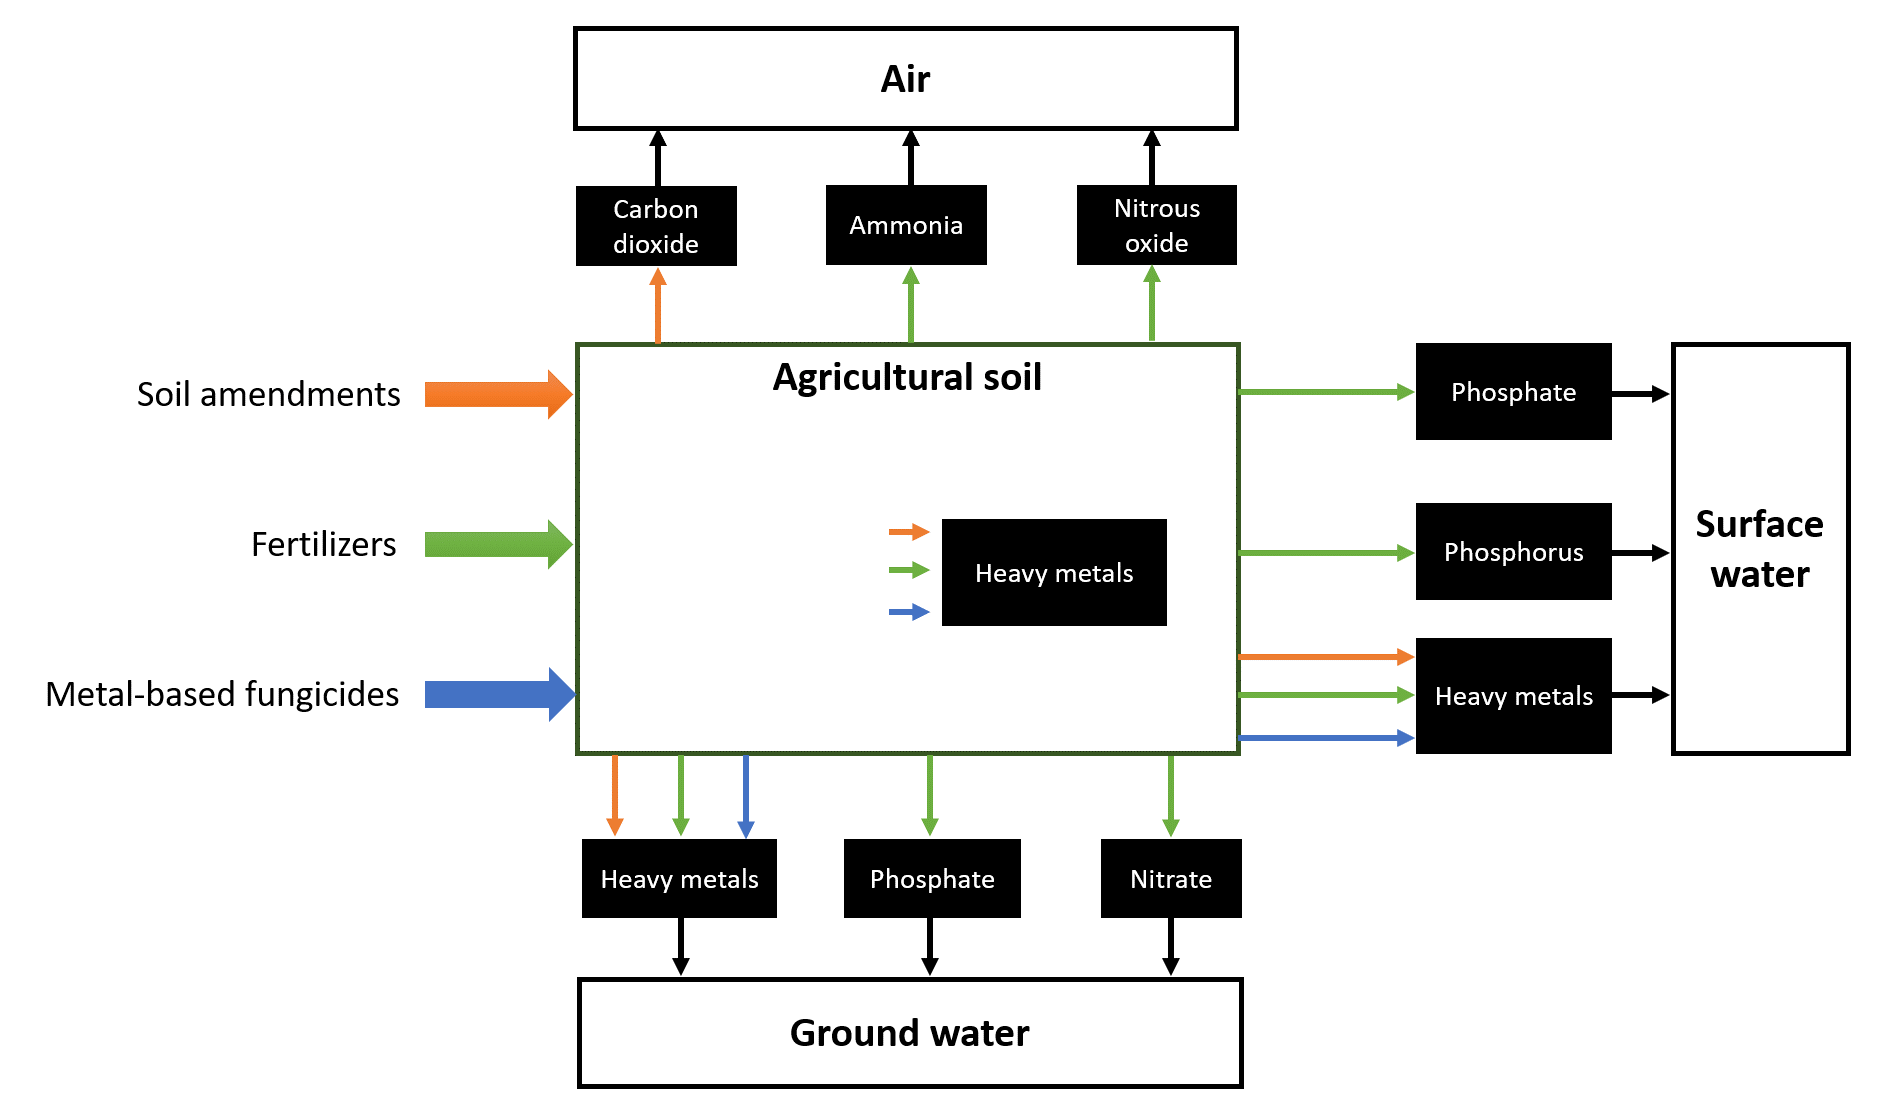
\includegraphics[width=0.95\linewidth]{Figures/agec_lci_emissions} 

}

\caption{Emissions Computed by AGEC-LCI}\label{fig:agec-lci-emissions}
\end{figure}

A state of the art analysis of the models for computing direct field emission from fertilizers, pesticides and soil amendments was carried out. Acknowledging that agricultural emissions are site- and time dependent, a parsimonious approach was considered for the selection of the models (Table \ref{tab:agec-models}). See \protect\hyperlink{selected-methods}{Section} \ref{selected-methods} for more details on the selected models.

\begin{longtable}[]{@{}llllll@{}}
\caption{\label{tab:agec-models} Selected models for calculating agricultural emissions and comparison with LCI databases}\tabularnewline
\toprule
\begin{minipage}[b]{0.12\columnwidth}\raggedright
Emission\strut
\end{minipage} & \begin{minipage}[b]{0.16\columnwidth}\raggedright

\includegraphics{Figures/agri-footprint.png} \href{https://www.agri-footprint.com/}{agri footprint} \citep{durlinger2017}\strut
\end{minipage} & \begin{minipage}[b]{0.12\columnwidth}\raggedright

\includegraphics{Figures/ecoinvent.png} \href{https://www.ecoinvent.org/}{ecoinvent v3} \citep{nemecek2011}\strut
\end{minipage} & \begin{minipage}[b]{0.13\columnwidth}\raggedright

\includegraphics{Figures/agribalyse.png} \href{https://www.ademe.fr/en/expertise/alternative-approaches-to-production/agribalyse-program}{AGRIBALYSE ®} \citep{Koch2015}\strut
\end{minipage} & \begin{minipage}[b]{0.12\columnwidth}\raggedright

\includegraphics{Figures/WFLDB.png} \href{https://quantis-intl.com/tools/databases/wfldb-food/}{WFLDB} \citep{nemecek2014}\strut
\end{minipage} & \begin{minipage}[b]{0.17\columnwidth}\raggedright
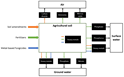
\includegraphics{Figures/agec_lci_logo.png} AGEC-LCI\strut
\end{minipage}\tabularnewline
\midrule
\endfirsthead
\toprule
\begin{minipage}[b]{0.12\columnwidth}\raggedright
Emission\strut
\end{minipage} & \begin{minipage}[b]{0.16\columnwidth}\raggedright

\includegraphics{Figures/agri-footprint.png} \href{https://www.agri-footprint.com/}{agri footprint} \citep{durlinger2017}\strut
\end{minipage} & \begin{minipage}[b]{0.12\columnwidth}\raggedright

\includegraphics{Figures/ecoinvent.png} \href{https://www.ecoinvent.org/}{ecoinvent v3} \citep{nemecek2011}\strut
\end{minipage} & \begin{minipage}[b]{0.13\columnwidth}\raggedright

\includegraphics{Figures/agribalyse.png} \href{https://www.ademe.fr/en/expertise/alternative-approaches-to-production/agribalyse-program}{AGRIBALYSE ®} \citep{Koch2015}\strut
\end{minipage} & \begin{minipage}[b]{0.12\columnwidth}\raggedright

\includegraphics{Figures/WFLDB.png} \href{https://quantis-intl.com/tools/databases/wfldb-food/}{WFLDB} \citep{nemecek2014}\strut
\end{minipage} & \begin{minipage}[b]{0.17\columnwidth}\raggedright
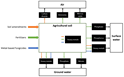
\includegraphics{Figures/agec_lci_logo.png} AGEC-LCI\strut
\end{minipage}\tabularnewline
\midrule
\endhead
\begin{minipage}[t]{0.12\columnwidth}\raggedright
Ammonia (NH\textsubscript{3})\strut
\end{minipage} & \begin{minipage}[t]{0.16\columnwidth}\raggedright
IPCC (2006)\strut
\end{minipage} & \begin{minipage}[t]{0.12\columnwidth}\raggedright
Agrammon (Tier 3 methodology for Switzerland)\strut
\end{minipage} & \begin{minipage}[t]{0.13\columnwidth}\raggedright
EMEP Tier 2 (EEA 2009)\strut
\end{minipage} & \begin{minipage}[t]{0.12\columnwidth}\raggedright
EMEP Tier 2 (EEA 2013)\strut
\end{minipage} & \begin{minipage}[t]{0.17\columnwidth}\raggedright
EMEP Tier 2 (EEA 2009 \& EEA 2013)\strut
\end{minipage}\tabularnewline
\begin{minipage}[t]{0.12\columnwidth}\raggedright
Nitrous oxide (N\textsubscript{2}O)\strut
\end{minipage} & \begin{minipage}[t]{0.16\columnwidth}\raggedright
IPCC (2006)\strut
\end{minipage} & \begin{minipage}[t]{0.12\columnwidth}\raggedright
IPCC (2006) crops: Tier 1 animals: Tier 2\strut
\end{minipage} & \begin{minipage}[t]{0.13\columnwidth}\raggedright
IPCC (2006) crops: Tier 1 animals: Tier 2\strut
\end{minipage} & \begin{minipage}[t]{0.12\columnwidth}\raggedright
IPCC (2006) crops: Tier 1 animals: Tier 2\strut
\end{minipage} & \begin{minipage}[t]{0.17\columnwidth}\raggedright
"IPCC (2006) crops: Tier 1\textsuperscript{(a)}\strut
\end{minipage}\tabularnewline
\begin{minipage}[t]{0.12\columnwidth}\raggedright
Nitrate (NO\textsubscript{3}\textsuperscript{-})\strut
\end{minipage} & \begin{minipage}[t]{0.16\columnwidth}\raggedright
IPCC (2006)\strut
\end{minipage} & \begin{minipage}[t]{0.12\columnwidth}\raggedright
Europe: SALCA-Nitrate (Richner et al.~2014), Other countries: SQCB (Faist et al, 2009)\strut
\end{minipage} & \begin{minipage}[t]{0.13\columnwidth}\raggedright
Annual French crops: COMIFER 2001 adjusted (Tailleur et al.~2012),Permanent crops: SQCB (Faist et al, 2009)\strut
\end{minipage} & \begin{minipage}[t]{0.12\columnwidth}\raggedright
Europe: SALCA-Nitrate (Richner et al.~2014), Other countries: SQCB (Faist et al, 2009)\strut
\end{minipage} & \begin{minipage}[t]{0.17\columnwidth}\raggedright
SQCB (Faist et al, 2009)\strut
\end{minipage}\tabularnewline
\begin{minipage}[t]{0.12\columnwidth}\raggedright
Phosphorus (P,PO\textsubscript{4}\textsuperscript{3-})\strut
\end{minipage} & \begin{minipage}[t]{0.16\columnwidth}\raggedright
(Struijs, Beusen, Zwart, \& Huijbregts, 2011)\strut
\end{minipage} & \begin{minipage}[t]{0.12\columnwidth}\raggedright
SALCA-P (Prasuhn, 2006)\strut
\end{minipage} & \begin{minipage}[t]{0.13\columnwidth}\raggedright
SALCA-P (Prasuhn, 2006)\strut
\end{minipage} & \begin{minipage}[t]{0.12\columnwidth}\raggedright
SALCA-P (Prasuhn, 2006)\strut
\end{minipage} & \begin{minipage}[t]{0.17\columnwidth}\raggedright
SALCA-P (Prasuhn, 2006)\strut
\end{minipage}\tabularnewline
\begin{minipage}[t]{0.12\columnwidth}\raggedright
Heavy metals (Cd, Cr, Cu, Hg, Ni, Pb, Zn)\strut
\end{minipage} & \begin{minipage}[t]{0.16\columnwidth}\raggedright
(Mels et al., 2008, Romkens \& Rietra, 2008, Nemecek \& Schnetzer, 2012)\strut
\end{minipage} & \begin{minipage}[t]{0.12\columnwidth}\raggedright
SALCA method (Freiermuth, 2006)\strut
\end{minipage} & \begin{minipage}[t]{0.13\columnwidth}\raggedright
SALCA method (Freiermuth, 2006)\strut
\end{minipage} & \begin{minipage}[t]{0.12\columnwidth}\raggedright
SALCA method (Freiermuth, 2006)\strut
\end{minipage} & \begin{minipage}[t]{0.17\columnwidth}\raggedright
SALCA method (Freiermuth, 2006)\strut
\end{minipage}\tabularnewline
\begin{minipage}[t]{0.12\columnwidth}\raggedright
Methane (CH\textsubscript{4})\strut
\end{minipage} & \begin{minipage}[t]{0.16\columnwidth}\raggedright
Dutch National Inventory Reports\strut
\end{minipage} & \begin{minipage}[t]{0.12\columnwidth}\raggedright
IPCC (2006) Tier 2\strut
\end{minipage} & \begin{minipage}[t]{0.13\columnwidth}\raggedright
IPCC (2006) Tier 2\strut
\end{minipage} & \begin{minipage}[t]{0.12\columnwidth}\raggedright
IPCC (2006) Tier 2\strut
\end{minipage} & \begin{minipage}[t]{0.17\columnwidth}\raggedright
-\strut
\end{minipage}\tabularnewline
\begin{minipage}[t]{0.12\columnwidth}\raggedright
Synthetic pesticides\strut
\end{minipage} & \begin{minipage}[t]{0.16\columnwidth}\raggedright
100 \% of the substance emitted to agricultural soil\strut
\end{minipage} & \begin{minipage}[t]{0.12\columnwidth}\raggedright
100 \% of the substance emitted to agricultural soil\strut
\end{minipage} & \begin{minipage}[t]{0.13\columnwidth}\raggedright
100 \% of the substance emitted to agricultural soil\strut
\end{minipage} & \begin{minipage}[t]{0.12\columnwidth}\raggedright
100 \% of the substance emitted to soil\textsuperscript{(b)}\strut
\end{minipage} & \begin{minipage}[t]{0.17\columnwidth}\raggedright
-\strut
\end{minipage}\tabularnewline
\bottomrule
\end{longtable}

(a): The AGEC-LCI tool does not compute enteric emissions of livestock.

(b): Rule followed in the first and second release of the WFLDB. The third release will follow the rules defined in Glasgow workshops \citep{nemecek2014}.

\hypertarget{instructions}{%
\chapter{Instructions for use}\label{instructions}}

\hypertarget{step-1}{%
\subsubsection*{Step 1}\label{step-1}}
\addcontentsline{toc}{subsubsection}{Step 1}

Unzip the compressed folder AGEC-LCI\_v1\_0.zip, then open the file AGEC-LCI\_v1\_0.xlsm (Figure \ref{fig:agec-icon}).

\begin{figure}[ht]

{\centering 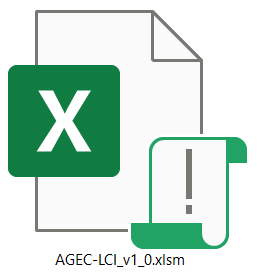
\includegraphics[width=0.15\linewidth]{Figures/agec_lci_icon} 

}

\caption{AGEC-LCI is stored in a macro-enabbled workbook}\label{fig:agec-icon}
\end{figure}

\hypertarget{step-2}{%
\subsubsection*{Step 2}\label{step-2}}
\addcontentsline{toc}{subsubsection}{Step 2}

Click on the Launch AGEC-LCI user interface button at the top of README-RUN worksheet of AGEC-LCI\_v1\_0.xlsm (Figure \ref{fig:agec-lci-step1}).

\begin{figure}[ht]

{\centering 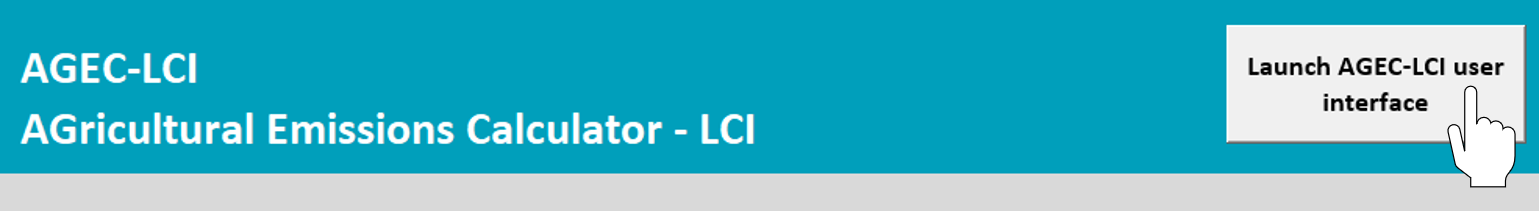
\includegraphics[width=0.85\linewidth]{Figures/agec_lci_step1} 

}

\caption{Launch AGEC-LCI user interface}\label{fig:agec-lci-step1}
\end{figure}

\hypertarget{step-3}{%
\subsubsection*{Step 3}\label{step-3}}
\addcontentsline{toc}{subsubsection}{Step 3}

The AGEC-LCI user interface will be displayed (Figure \ref{fig:agec-lci-step2}).

\begin{figure}[ht]

{\centering 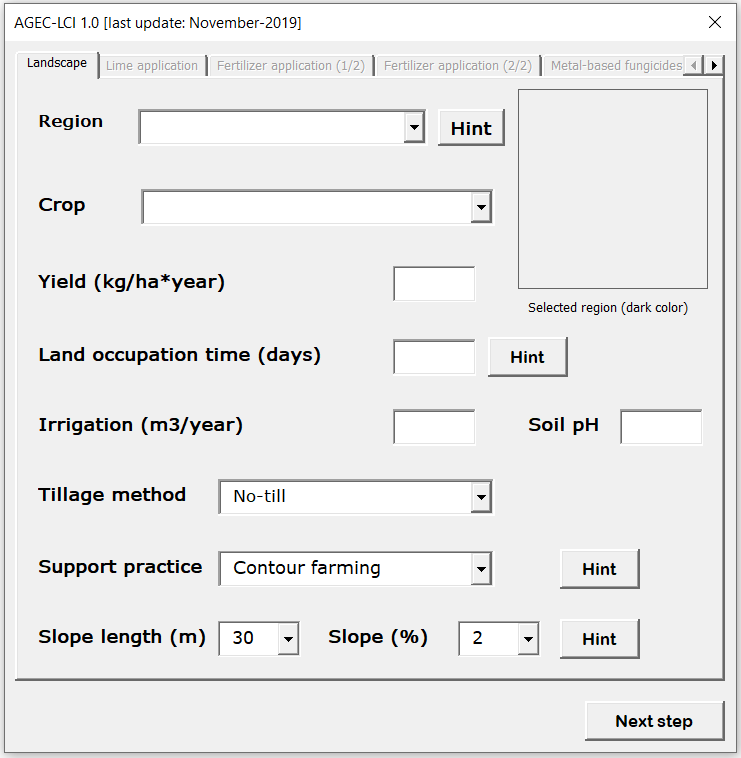
\includegraphics[width=0.65\linewidth]{Figures/agec_lci_step2} 

}

\caption{AGEC-LCI user interface}\label{fig:agec-lci-step2}
\end{figure}

AGEC-LCI allows the user to select inputs from a database composed of 25 crops, 42 fertilizers, 6 metal-based fungicides and the pedo-climatic characteristics of 5 French regions according to data from AGRIBALYSE \citep{Koch2015}. Furthermore, the user is allowed to add crops, regions and other inputs not available in the accompanying database.

\hypertarget{step-4}{%
\subsubsection*{Step 4}\label{step-4}}
\addcontentsline{toc}{subsubsection}{Step 4}

You will be asked to give a short name for your current project. It is advised to give a short and meaningful name, because it will be part of the name of the reports and the process generated (Figure \ref{fig:agec-lci-step3}). Click OK to finish the computations.

\begin{figure}[ht]

{\centering 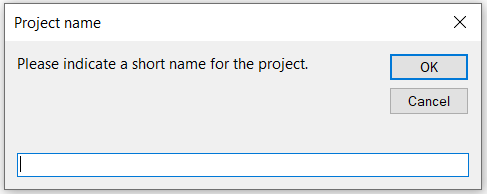
\includegraphics[width=6.76in]{Figures/agec_lci_step3} 

}

\caption{Name your current project}\label{fig:agec-lci-step3}
\end{figure}

\hypertarget{step-5}{%
\subsubsection*{Step 5}\label{step-5}}
\addcontentsline{toc}{subsubsection}{Step 5}

Three reports will be generated and stored under the Results folder accompanying this tool (Figure \ref{fig:agec-lci-step4}). The Results folder will be automatically open at the end of the computation.

\begin{itemize}
\item
  \textbf{Report\_Project\_Name\_YYYY-MM-DD.xlsx}: Contains the user's inputs and the calculated emissions. The aim of this report is to keep track of the inputs that need to be entered by the LCA practitioner into a LCA software.
\item
  \textbf{Report\_olca\_Project\_Name\_YYYY-MM-DD.xlsx}: Reports the calculated emissions in an Excel file compatible with openLCA. The importation of this report was tested with openLCA 1.9.0, and the procedure is described in \protect\hyperlink{import-olca}{Section} \ref{import-olca}.
\item
  \textbf{Report\_SimaPro\_Project\_Name\_YYYY-MM-DD.csv}: Reports the calculated emissions in a csv file compatible with SimaPro. The importation of this csv file was tested with SimaPro 8.5.2.2, it is not guaranteed that it will work in previous versions the software. The procedure for importing this file is described in \protect\hyperlink{import-simapro}{Section} \ref{import-simapro}.
\end{itemize}

\begin{figure}[ht]

{\centering 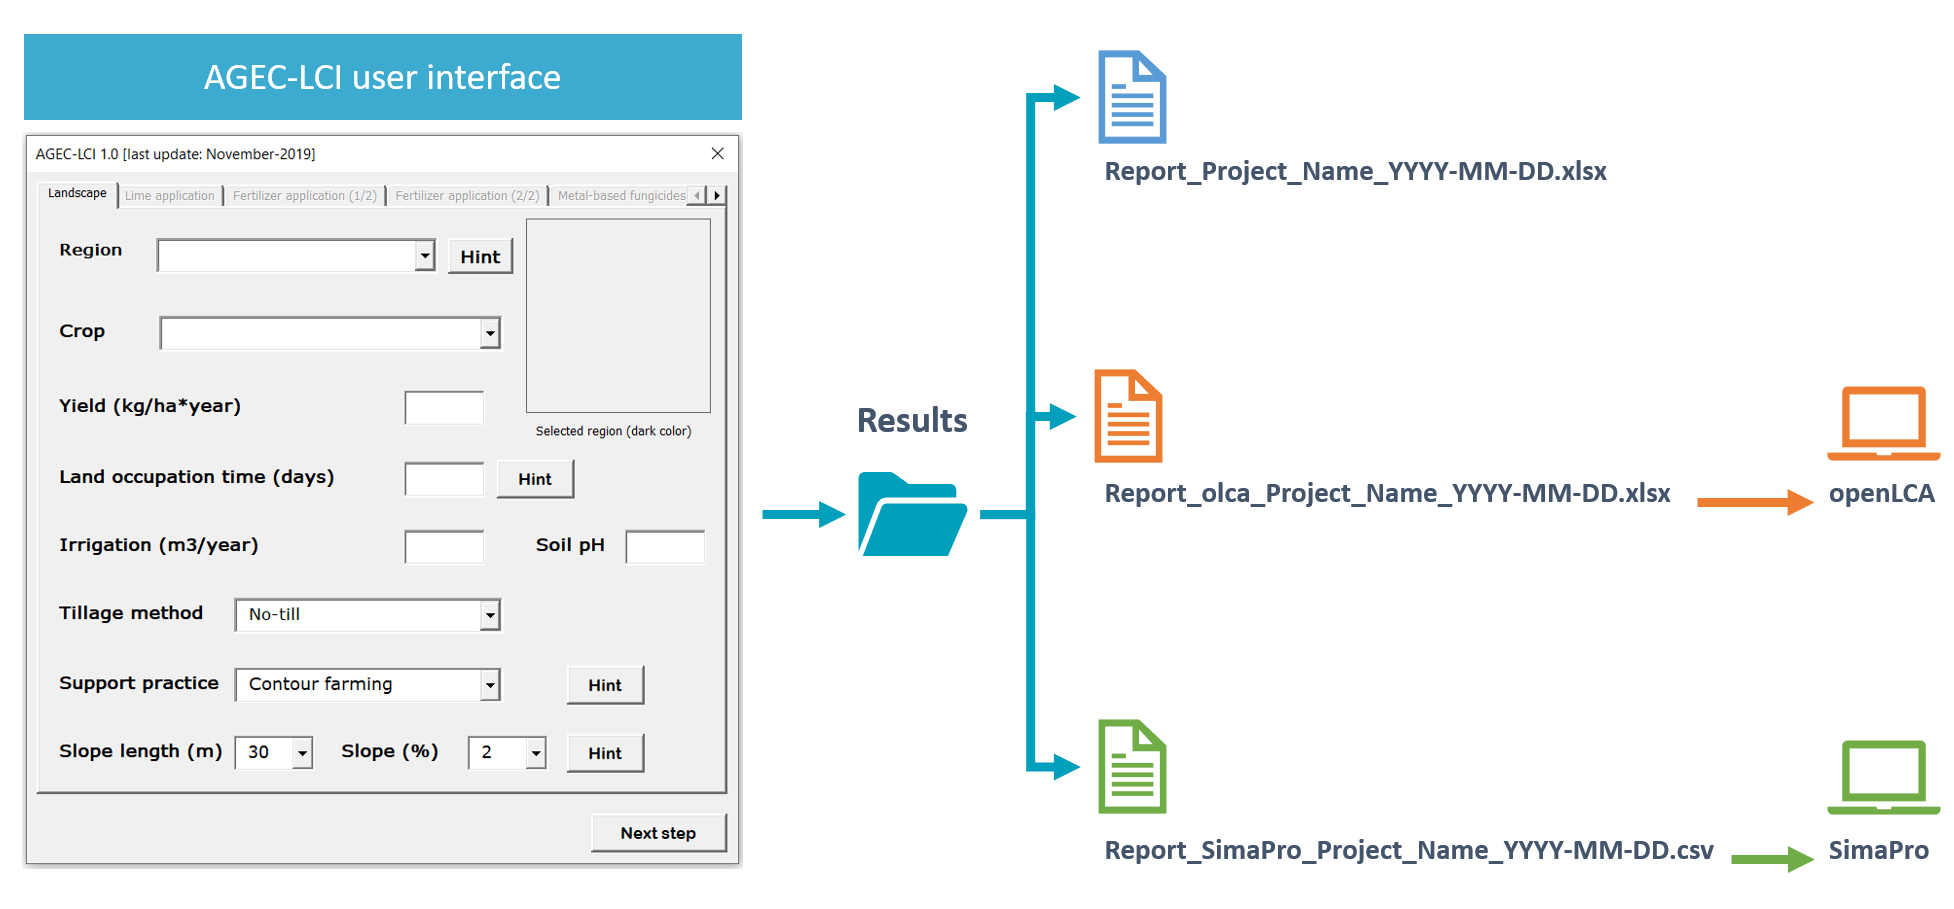
\includegraphics[width=0.95\linewidth]{Figures/age_lci_user_interface} 

}

\caption{Files generated by AGEC-LCI}\label{fig:agec-lci-step4}
\end{figure}

\hypertarget{importing-agec-lci-reports-into-lca-software}{%
\chapter{Importing AGEC-LCI reports into LCA software}\label{importing-agec-lci-reports-into-lca-software}}

AGEC-LCI generates reports that can be directly imported into LCA software such as \href{http://www.openlca.org/openlca/}{openLCA} and \href{https://simapro.com/}{SimaPro}, which greatly reduces the time required for computing the impact of emissions resulting from soil amendments, fertilizers and metal-based fungicides.

\hypertarget{import-olca}{%
\section{openLCA}\label{import-olca}}

\begin{enumerate}
\def\labelenumi{\arabic{enumi}.}
\item
  Activate your working database
\item
  Under \emph{File}, select import.
\item
  Select the \emph{Excel} file format and click on Next (Figure \ref{fig:olca-step1}).
\end{enumerate}

\begin{figure}[ht]

{\centering 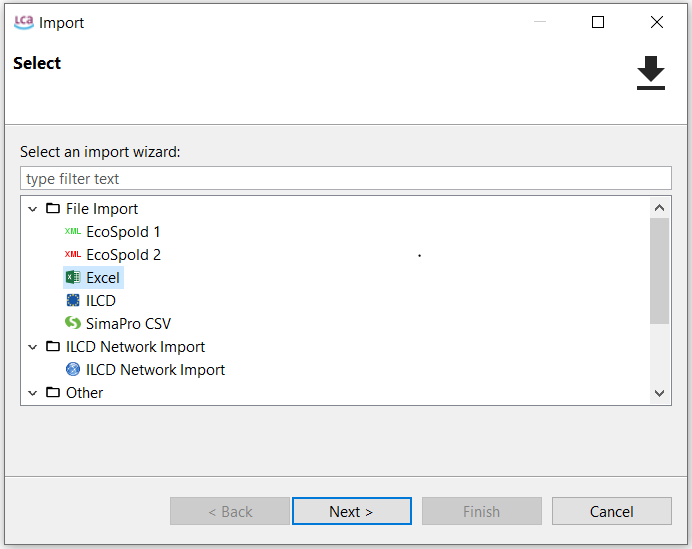
\includegraphics[width=0.7\linewidth]{Figures/olca_step1} 

}

\caption{Importing an Excel file into openLCA}\label{fig:olca-step1}
\end{figure}

\begin{enumerate}
\def\labelenumi{\arabic{enumi}.}
\setcounter{enumi}{3}
\item
  Find the \emph{AGEC-LCI report in Excel format} you would like to import. The name of the AGEC-LCI report compatible with openLCA follows the pattern ``Report\_olca\_Project\_Name\_YYYY-MM-DD.xlsx''. Of course, you can rename this file prior to its importation into openLCA.
\item
  Select the file to be imported and click on finish (Figure \ref{fig:olca-step2}).
\end{enumerate}

\begin{figure}[ht]

{\centering 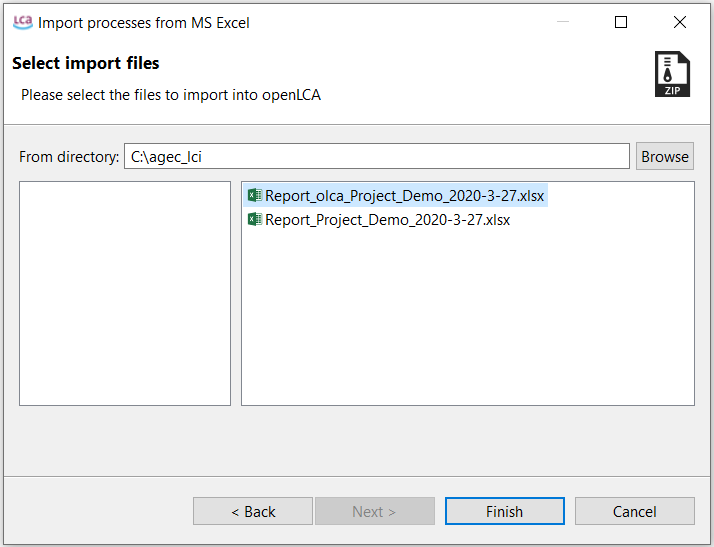
\includegraphics[width=0.7\linewidth]{Figures/olca_step2} 

}

\caption{Selecting the file to be imported}\label{fig:olca-step2}
\end{figure}

\begin{enumerate}
\def\labelenumi{\arabic{enumi}.}
\setcounter{enumi}{5}
\tightlist
\item
  After the importation, a child category AGEC-LCI will be created under Processes and Flows from the navigation panel (Figure \ref{fig:olca-step3}).
\end{enumerate}

\begin{figure}[ht]

{\centering 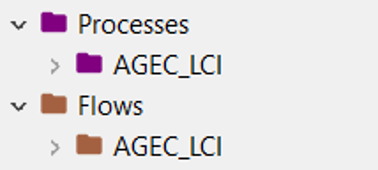
\includegraphics[width=0.4\linewidth]{Figures/olca_step3} 

}

\caption{Child categories added to Processes and Flows}\label{fig:olca-step3}
\end{figure}

\hypertarget{import-simapro}{%
\section{SimaPro}\label{import-simapro}}

\begin{enumerate}
\def\labelenumi{\arabic{enumi}.}
\item
  Open your project
\item
  Under \emph{File}, select import.
\item
  Click on Add.
\item
  Select the csv file for importing (Figure \ref{fig:simapro-step1}).
\end{enumerate}

\begin{figure}[ht]

{\centering 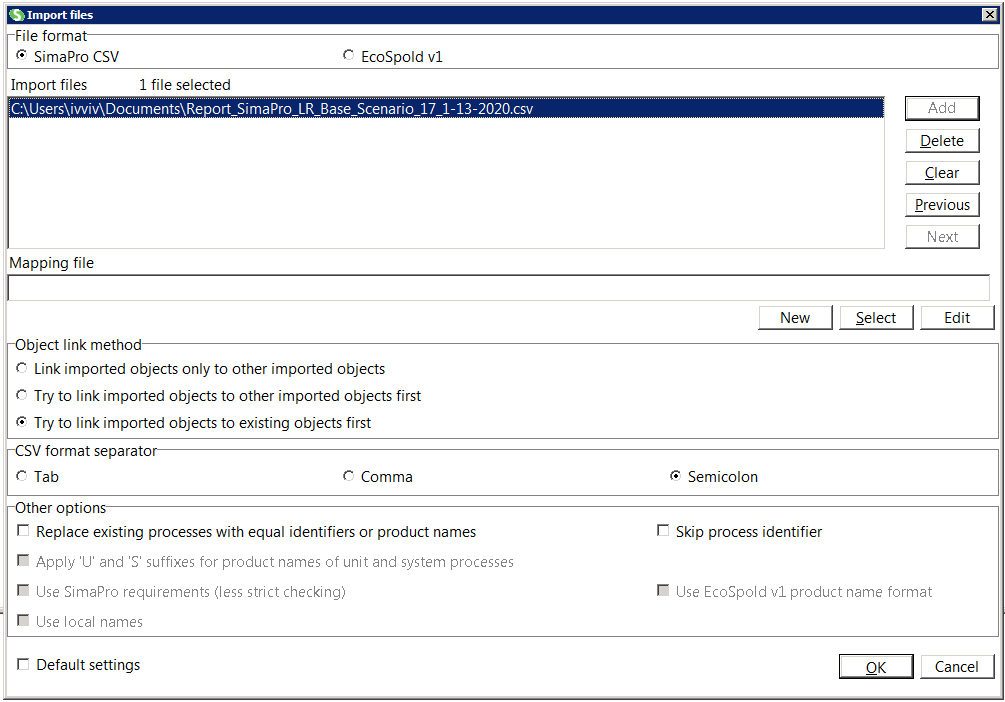
\includegraphics[width=0.85\linewidth]{Figures/simapro_step1} 

}

\caption{Importing a csv file into SimaPro}\label{fig:simapro-step1}
\end{figure}

\begin{enumerate}
\def\labelenumi{\arabic{enumi}.}
\setcounter{enumi}{4}
\item
  Click OK to launch the importation.
\item
  After the importation, a child category AGEC will be created under Processes/Use/Others (Figure \ref{fig:simapro-step2}).
\end{enumerate}

\begin{figure}[ht]

{\centering 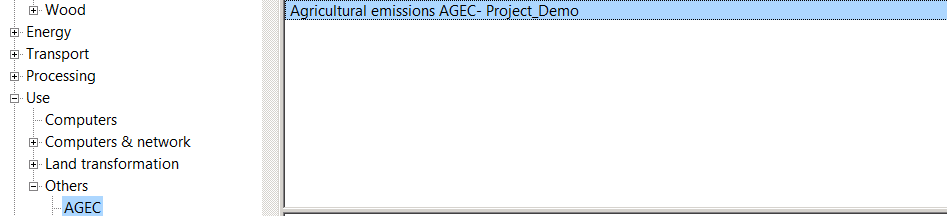
\includegraphics[width=0.85\linewidth]{Figures/simapro_step2} 

}

\caption{Child category added after importation}\label{fig:simapro-step2}
\end{figure}

\textbf{Notes:}

\begin{itemize}
\item
  The default name of the flow generated by AGEC-LCI is \emph{Agricultural emissions, AGEC}.
\item
  The default name of the process is composed by concatenation of the strings \emph{``Agricultural emissions, AGEC-LCI-''} and \emph{``Your Project Name''}, which you entered at step 3 of the \protect\hyperlink{instructions}{instructions for use}.
\end{itemize}

\hypertarget{selected-methods}{%
\chapter{Selected methods}\label{selected-methods}}

\hypertarget{soil-loss}{%
\section{Soil loss}\label{soil-loss}}

In line with the AGRIBALYSE® methodology \citep{Koch2015}, soil loss was estimated by applying the USDA RUSLE equation.

\[A = R\cdot K \cdot L \cdot S \cdot C \cdot P \cdot f\]

Where:

\begin{itemize}
\item
  \emph{A}: computed spatial and temporal average soil loss per unit area {[}t·ha\textsuperscript{-1}·yr\textsuperscript{-1}{]}
\item
  \emph{R}: rainfall-runoff erosivity factor
\item
  \emph{K}: soil erodibility factor
\item
  \emph{L}: slope length factor
\item
  \emph{S}: slope steepness factor
\item
  \emph{C}: cover-management factor
\item
  \emph{P}: support practice factor
\item
  \emph{f}: acre to hectare conversion factor (equal to 2.47)
\end{itemize}

The AGRIBALYSE ® program computed \emph{R} and \emph{K} parameters according to six principal regions of France: central, north, north-east, west, south and south-west. Furthermore, climate and soil profiles were defined for each region \citep{Koch2015}.

\hypertarget{emissions-of-ammonia-nh3-to-the-air}{%
\section{\texorpdfstring{Emissions of ammonia (NH\textsubscript{3}) to the air}{Emissions of ammonia (NH3) to the air}}\label{emissions-of-ammonia-nh3-to-the-air}}

In keeping with the AGRIBALYSE® methodology \citep{Koch2015}, emissions of NH\textsubscript{3} from organic fertilizers were calculated by applying the \citet{emep-eea2009} Tier 2. While the emissions of NH\textsubscript{3} resulting from the application of mineral fertilizers were calculated according to the \citet{emep-eea2013} Tier 2, which is in line with the World Food LCA Database (WFLDB) \citep{nemecek2014}. This allowed to consider the effect of both temperature and soil pH in the computation of NH\textsubscript{3} emissions.

The NH\textsubscript{3} emissions were calculated according to the following equation:

\[NH_3=\frac{17}{14} \cdot \sum_{m=1}^{M}(EF_a \cdot p + EF_b \cdot (1-p)) \cdot N \]

Where:

\begin{itemize}
\item
  \emph{NH\textsubscript{3}}: ammonia emissions after mineral fertilizer application {[}kg NH\textsubscript{3}{]}
\item
  \emph{m}: fertilizer type (M: number of fertilizer types)
\item
  \emph{EF\textsubscript{a}}: emission factor on soils with pH ≤ 7 {[}kg NH\textsubscript{3}-N/Kg N{]}
\item
  \emph{EF\textsubscript{b}}: emission factor on soils with pH \textgreater{} 7 {[}kg NH\textsubscript{3}-N/Kg N{]}
\item
  \emph{p}: fraction of soils with pH ≤ 7 {[}\%/100{]}
\item
  \emph{N}: fertilizer application {[}kg N{]}
\item
  \emph{17/14} is the conversion factor from N to NH\textsubscript{3}.
\end{itemize}

The above equation was simplified by considering that only one value of pH is reported for a given plot, which implies assuming that the pH is homogeneous in the studied agricultural field. In the equation below, \emph{i} can take the values \emph{EF\textsubscript{a}} or \emph{EF\textsubscript{b}}, whether the pH is below or above 7.\\
\[NH_3=\frac{17}{14} \cdot \sum_{m=1}^{M} EF_i \cdot N\]

\hypertarget{emissions-of-nitrogen-oxides-noxnono2-to-the-air}{%
\section{\texorpdfstring{Emissions of nitrogen oxides (NOx,NO,NO\textsubscript{2}) to the air}{Emissions of nitrogen oxides (NOx,NO,NO2) to the air}}\label{emissions-of-nitrogen-oxides-noxnono2-to-the-air}}

Nitrogen oxides result principally from the nitrification process. In line with the AGRIBALYSE® methodology \citep{Koch2015} and the WFLDB \citep{nemecek2014}, the \citet{emep-eea2009} Tier 1 was applied to calculate nitric oxide emission generated from the application of organic and mineral fertilizers. Regardless of the type of fertilizer (i.e., organic or mineral) the same emission factor is used:

\begin{itemize}
\tightlist
\item
  \textbf{Emission factor for NOx-N}: 0.012 kg NOx-N/kg N applied
\end{itemize}

Prior to the computation of NO emissions, N volatized as NH\textsubscript{3} was substracted from the amount of N applied.

In ecoinvent, nitrogen oxide emissions are calculated with respect to NO\textsubscript{2}. In consequence, a conversion factor of 46/14 was applied to the calculated emissions in terms of N.

\hypertarget{nitrate-no3--leaching-to-ground-water}{%
\section{\texorpdfstring{Nitrate (NO\textsubscript{3}\textsuperscript{-}) leaching to ground water}{Nitrate (NO3-) leaching to ground water}}\label{nitrate-no3--leaching-to-ground-water}}

\citet{faist2009} employed a simple regression model from Willigen (2000) to calculate nitrate leaching to groundwater in the context of the \emph{Sustainability Quick Check for Biofuels Project}. The main limitation of the SQCB-NO\textsubscript{3} model is that it does not account for soil hydrological and biochemical processes. In consequence, the output of this model must be considered as an estimate of nitrate leaching. Nevertheless, the SQCB-NO\textsubscript{3} model has been applied in AGRIBALYSE® \citep{Koch2015}, WFLDB \citep{nemecek2014} and ecoinvent \citep{nemecek2011} to calculate nitrate leaching in non-European agricultural fields.

The SQCB-NO3 model was selected over the SALCA-nitrate model because the former was used by AGRIBALYSE ® to calculate nitrate leaching in vineyard fields, which is a research interest of the authors. Furthermore, this model allows to consistently compute nitrate emissions for other crops, and it facilitates updating the VBA application.

Nitrate emissions were calculated according to the following regression model \citep{faist2009}:

\[N=21.37 + \frac{P}{c \cdot L} \Big[0.0037 \cdot S + 0.0000601 \cdot N_{org} - 0.00362 \cdot U  \Big]\]

Where:

\begin{itemize}
\item
  \emph{N}: quantity of nitrogen leached {[}kg N·ha\textsuperscript{-1}·year\textsuperscript{-1}{]}
\item
  \emph{P}: precipitation and watering, in mm per year
\item
  \emph{c}: soil clay content, in basis 100
\item
  \emph{L}: rooting depth, in meters
\item
  \emph{S}: nitrogen supply, including crop residues {[}kg N·ha\textsuperscript{-1}{]}
\item
  \emph{N\textsubscript{org}}: quantity ot nitrogen in the soil organic matter {[}kg N·ha\textsuperscript{-1}{]}
\item
  \emph{U}: nitrogen uptake {[}kg N·ha\textsuperscript{-1}{]}
\end{itemize}

A conversion factor of 62/14 was applied to the calculated emissions of nitrate in terms of N.

\hypertarget{emissions-of-nitrous-oxide-n2o-to-air}{%
\section{\texorpdfstring{Emissions of nitrous oxide (N\textsubscript{2}O) to air}{Emissions of nitrous oxide (N2O) to air}}\label{emissions-of-nitrous-oxide-n2o-to-air}}

Nitrous oxide (N\textsubscript{2}O) results from nitrification and denitrification processes. The global warming potential (GWP) of N\textsubscript{2}O for a time horizon of 100 years is 310 times the GWP of CO\textsubscript{2} \citep{IPCC2006}.

N\textsubscript{2}O emissions were calculated according to the following equation \citep{IPCC2006}:

\[N_2O = \frac{44}{28} \cdot \bigg (0.01 \cdot \Big(N_{tot} + N_{cr} + \frac{14}{17} \cdot NH_3 + \frac{14}{46} \cdot NOx \Big) + 0.0075 \cdot \frac{14}{62} \cdot NO_3 \bigg)\]

Where:

\begin{itemize}
\item
  \emph{N\textsubscript{2}O}: emissions of nitrous oxide {[}kg N\textsubscript{2}O·ha\textsuperscript{-1}{]}
\item
  \emph{N\textsubscript{tot}}: total nitrogen in mineral and organic fertilizer {[}kg N·ha\textsuperscript{-1}{]}
\item
  \emph{N\textsubscript{cr}}: nitrogen contained in the crop residues {[}kg N·ha\textsuperscript{-1}{]}
\item
  \emph{NH\textsubscript{3}}: losses of nitrogen in the form of ammonia {[}kg NH\textsubscript{3}·ha\textsuperscript{-1}{]}
\item
  \emph{NOx}: losses of nitrogen in the form of nitrogen oxides {[}kg NO\textsubscript{2}·ha\textsuperscript{-1}{]}
\item
  \emph{NO\textsubscript{3}}: losses of nitrogen in the form of nitrate {[}kg NO\textsubscript{3}·ha\textsuperscript{-1}{]}
\end{itemize}

\hypertarget{carbon-dioxide-co2-from-liming-and-urea-application}{%
\section{\texorpdfstring{Carbon dioxide (CO\textsubscript{2}) from liming and urea application}{Carbon dioxide (CO2) from liming and urea application}}\label{carbon-dioxide-co2-from-liming-and-urea-application}}

The aim of applying lime in agricultural soils is to decrease soil acidity and to improve plant development. The addition of carbonates by means of limestone or dolomite entails the dissolution of carbonate limes and the release of bicarbonate (2HCO\textsubscript{3}\textsuperscript{-}). Subsequently, the bicarbonate is transformed into CO\textsubscript{2} and water \citep{IPCC2006}.

In agreement with the AGRIBALYSE® methodology \citep{Koch2015}, the WFLDB \citep{nemecek2014}, and ecoinvent \citep{nemecek2011}, carbon dioxide emissions generated from the application of lime and urea were calculated according to \citet{IPCC2006} Tier 1. The calculated emissions are based on a worst-case approach because it is considered that the total amount of carbon is released in the form of CO\textsubscript{2}.

CO\textsubscript{2} emissions from lime application:

\[CO_2-C_{Emission}=M_{limestone} \cdot EF_{limestone} + M_{dolomite} \cdot EF_{dolomite}\]

Where:

\begin{itemize}
\item
  \emph{CO\textsubscript{2}-C\textsubscript{Emissions}}: C emissions from lime application, tonnes C·yr\textsuperscript{-1}
\item
  \emph{M}: annual amount of calcic limestone or dolomite, tonnes·yr\textsuperscript{-1}
\item
  \emph{EF}: emission factor, tonne of C·(tonne of limestone or dolomite)\textsuperscript{-1}
\end{itemize}

\begin{longtable}[]{@{}ll@{}}
\caption{\label{tab:carbon-dioxide-ef} EF-Emission factor (kg of C·kg of product\textsuperscript{-1})}\tabularnewline
\toprule
Product & EF\tabularnewline
\midrule
\endfirsthead
\toprule
Product & EF\tabularnewline
\midrule
\endhead
Limestone & 0.12\tabularnewline
Dolomite & 0.13\tabularnewline
Urea & 1.57\tabularnewline
\bottomrule
\end{longtable}

Finally, a factor of 44/12 is applied to transform the emissions in terms of carbon into emissions based on carbon dioxide.

\[CO_2= \frac{44}{12} \cdot CO_2-C_{Emission}\]

\hypertarget{phosphorous-emissions}{%
\section{Phosphorus emissions}\label{phosphorous-emissions}}

In agreement with the AGRIBALYSE® methodology \citep{Koch2015}, the WFLDB methodology \citep{nemecek2014} and the ecoinvent methodology \citep{nemecek2011}, emissions of phosphorous to water were calculated by applying the SALCA-P model \citep{prasuhn2006}.

The SALCA-P model computes three types of emissions to water according to the mechanism generating them:

\begin{itemize}
\tightlist
\item
  Phosphorus to river (emission by soil loss)
\item
  Phosphate to ground water (emission by leaching).
\item
  Phosphate to river (emission by run-off)
\end{itemize}

\hypertarget{phosphorus-to-river-emission-by-soil-loss}{%
\subsection{Phosphorus to river (emission by soil loss)}\label{phosphorus-to-river-emission-by-soil-loss}}

Emissions of phosphorus by soil loss were calculated according to the following equation \citep{prasuhn2006}:

\[P_E=A \cdot P_S \cdot F_R \cdot F_{SR} \cdot t\]
Where:

\begin{itemize}
\item
  \emph{P\textsubscript{E}}: phosphorus emitted by soil loss to rivers {[}kg.ha\textsuperscript{-1}.yr\textsuperscript{-1}{]}
\item
  \emph{A}: quantity of soil lost {[}kg.ha\textsuperscript{-1}.yr\textsuperscript{-1}{]}
\item
  \emph{t}: land occupation time (number of days/365)
\end{itemize}

\begin{longtable}[]{@{}llll@{}}
\caption{\label{tab:phosphorous-river} Parameters for calculating phosphorous emissions to river \citep{prasuhn2006}}\tabularnewline
\toprule
Parameter & Definition & Default value & Units\tabularnewline
\midrule
\endfirsthead
\toprule
Parameter & Definition & Default value & Units\tabularnewline
\midrule
\endhead
\emph{P\textsubscript{S}} & Phosphorous content in the upper part of the soil & 0.00095 & kg P·kg soil\textsuperscript{-1}\tabularnewline
\emph{F\textsubscript{R}} & Eroded particle enrichment factor & 1.86 & -\tabularnewline
\emph{F\textsubscript{SR}} & Fraction of soil lost that reaches the river & 0.2 & -\tabularnewline
\bottomrule
\end{longtable}

\hypertarget{phosphate-to-ground-water-emission-by-leaching}{%
\subsection{Phosphate to ground water (emission by leaching)}\label{phosphate-to-ground-water-emission-by-leaching}}

Leaching of phosphate to ground water was calculated according to the following equation \citep{prasuhn2006}:

\[P_L=P_{LM} \cdot F_{CSS} \cdot t\]

Where:

\begin{itemize}
\item
  \emph{P\textsubscript{L}}: leached phosphorus {[}kg.ha\textsuperscript{-1}.yr\textsuperscript{-1}{]}
\item
  \emph{P\textsubscript{LM}}: average quantity of phosphorus leached depending on the land occupation category {[}kg P.ha\textsuperscript{-1}.yr\textsuperscript{-1}{]}
\item
  \emph{F\textsubscript{CSS}}: correction factor for fertilization with slurry and/or sludge (see equation below)
\item
  \emph{t}: occupation time (number of days/365)
\end{itemize}

A conversion factor of 95/31 was applied to convert emissions of phosphorus into emissions of phosphate.

\[F_{CSS}=1+ \frac{0.2 \cdot (P_2O_{5-slurry\: and\: sludge})}{80}\]

\hypertarget{phosphate-to-river-emission-by-run-off}{%
\subsection{Phosphate to river (emission by run-off)}\label{phosphate-to-river-emission-by-run-off}}

Emissions of phosphate to river by run-off were calculated according to the following equation \citep{prasuhn2006}:

\[P_R=P_{RM} \cdot F_C \cdot F_S \cdot t\]

Where:

\begin{itemize}
\item
  \emph{P\textsubscript{R}}: phosphorus lost by run-off to the rivers {[}kg.ha\textsuperscript{-1}.yr\textsuperscript{-1}{]}
\item
  \emph{P\textsubscript{RM}}: average quantity of phosphorus lost by run-off depending on the land occupation category {[}kg P.ha\textsuperscript{-1}.yr\textsuperscript{-1}{]}
\item
  \emph{F\textsubscript{C}}: correction factor for the form of phosphorus applied (mineral, liquid/solid organic)
\item
  \emph{F\textsubscript{S}}: slope factor. F\textsubscript{S} = 0 if slope \textless{} 3\%, F\textsubscript{S}= 1, otherwise.
\item
  \emph{t}: occupation time (number of days/365)
\end{itemize}

\[F_C=1+ \frac{0.7 \cdot P_2O_{5-slurry\: and \: sludge} + 0.2 \cdot P_2O_{5-mineral \: fertilizer} + 0.4  \cdot P_2O_{5-manure\: and\: compost}}{80}\]

A conversion factor of 95/31 was applied to convert emissions of phosphorus into emissions of phosphate.

\hypertarget{heavy-metal-emissions-to-agricultural-soil-surface-water-and-ground-water}{%
\section{Heavy metal emissions to agricultural soil, surface water and ground water}\label{heavy-metal-emissions-to-agricultural-soil-surface-water-and-ground-water}}

Emissions of heavy metals to soil, ground and surface water are calculated based on a mass balance. The inputs considered are seeds, fertilizers, soil amendments, metal-based pesticides and air deposition. The outputs correspond to the emissions of trace metals into ground and surface water and the products harvested.

\hypertarget{heavy-metal-emissions-to-agricultural-soils}{%
\subsection{Heavy metal emissions to agricultural soils}\label{heavy-metal-emissions-to-agricultural-soils}}

The mass balance of trace metal \emph{(TM) x} in soil is calculated according to the following equation \citep{Koch2015}:

\[\Delta F_{TMx}=\sum_{SFPI_y}IN_y \cdot C_{y,x} - \Big (\sum_{PLR_z} OUT_z \cdot C_{z,x} \Big) \cdot Alloc_x \quad \forall x \in \{Cd,Cu,Zn,Pb,Ni,Cr,Hg\}\]

Where:

\begin{itemize}
\item
  \emph{ΔFTMx}: Flow into the soil of \emph{Trace Metal x (TMx)}
\item
  \emph{INy}: Quantity of input \emph{SFPIy} containing TMx:

  \begin{itemize}
  \item
    Seed
  \item
    Fertilizer (mineral, organic, farm, sludge)
  \item
    Pesticides
  \item
    Sundry Inputs
  \end{itemize}
\item
  \emph{Cy,x}: Content of \emph{TMx} in input \emph{SFPIy}
\item
  \emph{OUTz}: Quantity of output \emph{PLRz} carrying the trace metal \emph{TMx}

  \begin{itemize}
  \item
    Products harvested (including co-products and/or residues exported)
  \item
    Leaching to groundwater
  \item
    Run-off to surface water by soil loss
  \end{itemize}
\item
  \emph{Cz,x}: Content of \emph{TMx} in output PLRz
\item
  \emph{Alloc\textsubscript{x}}: Allocation factor for TMx output flow. This allocation factor only takes account of part of the output flows from the deposition of trace metals. The allocation is calculated for each trace metal:
\end{itemize}

\[Alloc_x = \frac{ \sum_{SFPIy}IN_y \cdot T_{y,x}}{ \sum_{SFPIy} IN_y \cdot T_{y,x} + Dep_x}\]

\hypertarget{heavy-metal-emissions-to-river}{%
\subsection{Heavy metal emissions to river}\label{heavy-metal-emissions-to-river}}

Trace metal emissions through erosion are calculated according to the following equation \citep{Koch2015}:

\[M_{erosion,TMx} = A \cdot S_{TMx} \cdot F_R \cdot F_{SR} \cdot t \cdot Alloc_x\]

Where:

\begin{itemize}
\item
  \emph{M\textsubscript{erosion,TM}x}: emission of trace metal x to river {[}kg·ha\textsuperscript{-1}·yr\textsuperscript{-1}{]}
\item
  \emph{A}: amount of soil lost {[}kg·ha\textsuperscript{-1}·yr\textsuperscript{-1}{]}
\item
  \emph{S\textsubscript{TMx}}: the content of trace metal x in the upper part of the soil
\item
  \emph{F\textsubscript{R}}: eroded particle enrichment factor
\item
  \emph{F\textsubscript{SR}}: fraction of soil lost which reaches the river
\item
  \emph{t}: land occupation time (number of days/365)
\item
  \emph{Alloc\textsubscript{x}}: allocation factor for trace metal x
\end{itemize}

The amount of soil lost was calculated by applying the RUSLE equation. An average concentration of trace metals depending on the soil use was considered. The eroded particle enrichment factor and the fraction of soil lost that reaches the river took the default values considered in the AGRIBALYSE® methodology \citep{Koch2015}. Please refer to \protect\hyperlink{phosphorous-emissions}{Section} \ref{phosphorous-emissions} to retrieve the last two parameters.

\hypertarget{heavy-metal-emissions-to-ground-water}{%
\subsection{Heavy metal emissions to ground water}\label{heavy-metal-emissions-to-ground-water}}

Trace metal emissions into ground water were calculated according to the following equation \citep{Koch2015}:

\[M_{leachng,TMx} = m_{leaching,TMx} \cdot Alloc_x\]

Where:

\begin{itemize}
\item
  \emph{M\textsubscript{leaching,TMx}}: emission of trace metal x to ground water {[}kg·ha\textsuperscript{-1}·yr\textsuperscript{-1}{]}
\item
  \emph{m\textsubscript{leaching,TMx}}: average emission of trace metal x to ground water {[}kg·ha\textsuperscript{-1}·yr\textsuperscript{-1}{]}
\item
  \emph{Alloc\textsubscript{x}}: allocation factor for trace metal x.
\end{itemize}

\bibliography{book.bib}


\end{document}
